\section{Experiments}
\label{sec:experiments}

\begin{table}
  \caption{Comparison of multilingual topic modeling methods. Multilingual anchoring scores higher in classification accuracy and topic coherence than \abr{mcta}.  \mtanchor does as well as multilingual anchoring on average, but a few users can achieve the best results for every metric.}
  \centering
  \scriptsize
  \begin{tabular}{llllllllll} \\
    & & \multicolumn{4}{c}{Classification accuracy} & \multicolumn{4}{c}{Topic coherence} \\
    \cmidrule(r){3-6} \cmidrule(r){7-10} 
    Dataset & Method & \abr{en-i} & \makecell{\abr{zh-i}\\\abr{si-i}} & \abr{en-c} & \makecell{\abr{zh-c}\\\abr{si-c}} & \abr{en-i} & \makecell{\abr{zh-i}\\\abr{si-i}} & \abr{en-e} & \makecell{\abr{zh-e}\\\abr{si-e}} \\
    \midrule 
    Wikipedia (\abr{en}-\abr{zh}) & Multilingual anchoring & 69.49\% & 71.24\% & 50.37\% & 47.76\% & 0.141 & 0.178 & 0.084 & 0.128  \\
    & \mtanchor (maximum) & \textbf{80.71}\% & \textbf{75.33}\% & \textbf{57.62}\% & \textbf{54.54}\% & \textbf{0.195} & \textbf{0.198} & \textbf{0.103} & \textbf{0.147} \\
    & \mtanchor (median) & 69.49\% & 71.44\% & 50.27\% & 47.22\% & 0.141 & 0.178 & 0.084 & 0.129\\
    & \abr{mcta} & 51.56\% & 33.35\% & 23.24\% & 39.79\% & 0.126 & 0.085 & 0.000 & 0.037  \\
    \midrule
    Amazon (\abr{en}-\abr{zh}) & Multilingual anchoring & \textbf{59.79}\% & \textbf{61.10}\% & \textbf{51.73}\% & \textbf{53.20}\% & \textbf{0.069} & \textbf{0.061} & \textbf{0.031} & \textbf{0.045} \\
    & \abr{mcta} & 49.53\% & 50.64\% & 50.27\% & 49.49\% & -0.028 & 0.019 & 0.017 & 0.011 \\
    \midrule 
    \abr{lorelei} (\abr{en}-\abr{si}) & Multilingual anchoring & \textbf{20.78}\% & \textbf{32.65}\% & \textbf{24.49}\% & \textbf{24.68}\% & 0.077 & 0.000 & 0.025 & n/a \\
    & \abr{mcta} & 12.99\% & 26.53\% & 4.08\% & 15.58\% & \textbf{0.132} & 0.000 & \textbf{0.036} & n/a  \\
  \end{tabular}
  \label{table:results}
\end{table}


The first dataset consists of Wikipedia articles: $11{,}043$ in English and $10{,}135$ in Chinese.  We shorten the articles to contain no more than three sections.  We lemmatize the English articles using WordNet Lemmatizer~\citep{bird-2009} and segment the Chinese articles using Stanford Core\abr{nlp}~\citep{manning-2014}.  For both languages, the articles fall under one of six categories: film, music, animals, politics, religion, and food.  

Another dataset consists of Amazon reviews: $53{,}558$ in English and $53{,}160$ in Chinese (mostly from Taiwan)~\citep{constant-2009}.  Each review has a rating, ranging from one to five.  Since about half of the reviews have a rating of five, we change the classification task to a binary problem by labeling reviews with rating of five as ``1'' and the rest as ``0''.  For the Wikipedia and Amazon datasets, the training-test split is set to 80:20.  For the Chinese-English dictionary, we use entries from MDBG.\footnote{\url{https://www.mdbg.net/chinese/dictionary?page=cc-cedict}.}

To test low-resource languages, we use data from the \abr{lorelei} Sinhalese language pack~\citep{strassel-2016}.  These language packs are created to develop technologies that can process data in low-resource languages.  In the pack, only a small subset of documents are labeled based on need type.\footnote{Documents in \abr{lorelei} language pack have multiple need types, but we have simplified the classification task by assigning only the first label to each document.}  So, we treat the classification task as a semi-supervised problem.  There are eight possible labels: evacuation, food supply, search/rescue, utilities, infrastructure, medical assistance, shelter, and water supply~\citep{strassel-2017}.  Out of the $1{,}100$ ($4{,}790$) English (Sinhalese) documents, only $77$ ($49$) of them have labels.  For each language, half of the labeled documents are in the training set and the other half are in the test set. For the Sinhalese-English dictionary, we use entries from the \abr{lorelei} Sinhalese language pack. 

We run experiments to evaluate three methods: multilingual anchoring, \mtanchor, and \abr{mcta} (Multilingual Cultural-common Topic Analysis)~\citep{shi-2016}.  We choose \abr{mcta} as a baseline because it is a recent work on multilingual topic models with readily available code and aligns topics using a bilingual dictionary.  We train models on multilingual anchoring and \abr{mcta} with twenty topics.  For \mtanchor, we initially show users twenty topics, but the final number of topics is their choice.  All methods are implemented in Python on a 2.3 GHz Intel Core i5 processor.

The data for the \mtanchor user study are the English-Chinese Wikipedia articles.  We invite twenty participants on Amazon Mechanical Turk (MTurk) to partake in the study.  Each user is given thirty minutes to interact with the interface.\footnote{Synopsis of user instructions: ``There are 11,000 English Wikipedia articles and 10,000 Chinese Wikipedia articles, which belong to one of six categories: film, music, animals, politics, religion, food.  Your goal is to find topics that can help classify documents within 30 minutes.''}  \mtanchor scales with the number of unique word types, rather than number of documents or number of words in the documents, so updates to the system take no longer than seven seconds on average.  We only approve HITs from workers who have completed the task for the first time.  After worker finishes the task, the interface provides a unique code for them to enter on MTurk.  These rules ensure fair assessment of workers' interaction with \mtanchor.

\begin{figure}
  \centering
  \subfloat{
    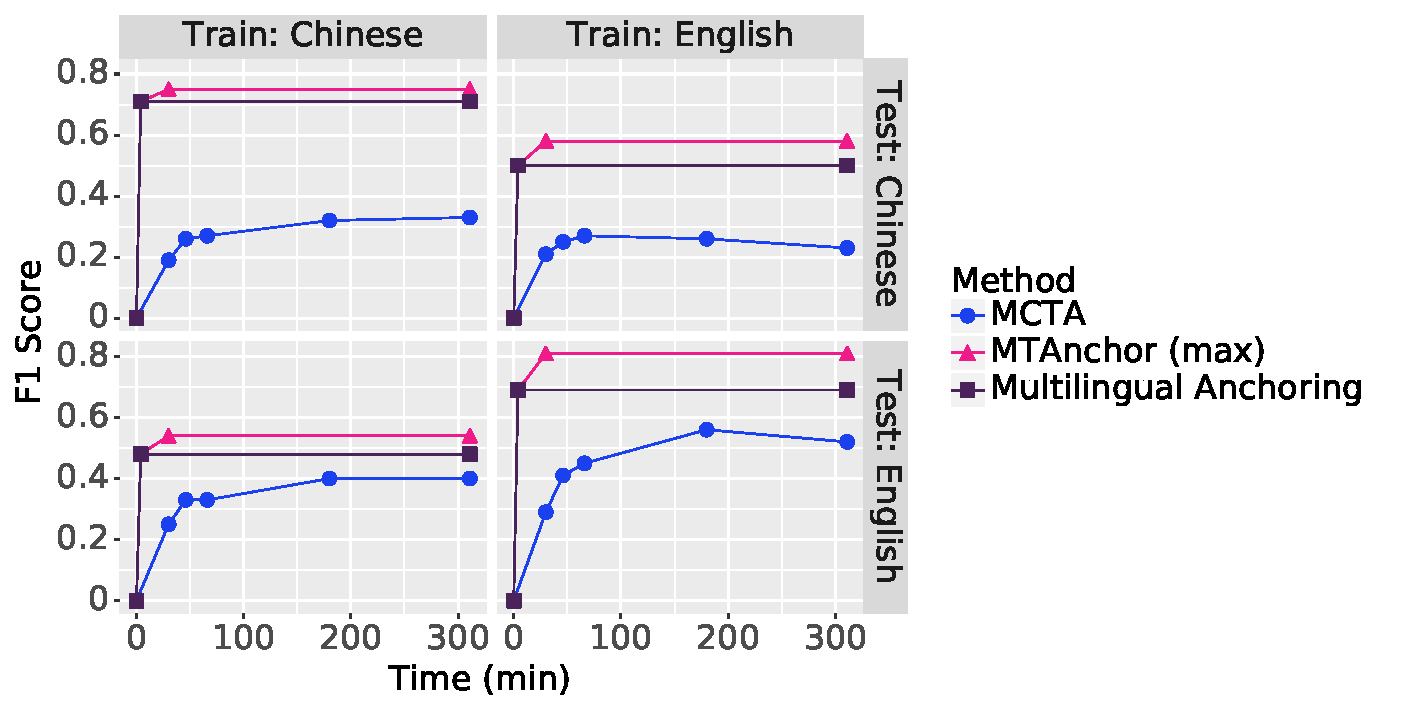
\includegraphics[width=0.8\textwidth]{methods_wiki.pdf}
  }
  \caption{Classification accuracy over time until \abr{mcta} converges. For the Wikipedia dataset, multilingual anchoring converges within 5 minutes, but \abr{mcta} takes 5 hours and 18 minutes to converge.  Multilingual anchoring outperforms \abr{mcta} in speed and classification accuracy.}
  \label{fig:convergence}
\end{figure}


\subsection{Evaluating multilingual topics}

Ideally, topic models should have topics that are \emph{interpretable} and \emph{useful} as classification features.  So, we primarily base evaluation on two measures: classification accuracy and topic coherence.  Measuring topic coherence considers both intrinsic and extrinsic scores~\citep{lau-2014}.  The difference between the two is the reference corpus.\footnote{Measuring topic coherence requires a reference corpus to sample lexical probabilities.} The intrinsic score uses the trained corpus itself, whereas the extrinsic score uses an external, larger dataset.  The Sinhalese extrinsic coherence scores are not available because a large reference corpus cannot be formed for low-resource languages.  By measuring both, we can evaluate the model's interpretability within a local and global context.   

We evaluate these metrics separately for each language: English~(\abr{en}), Chinese~(\abr{zh}), and Sinhalese~(\abr{si}).  To classify labels from topics, we use the same procedure as described in Section~\ref{sec:predict}.  Then, we measure intra-lingual (\abr{i}) and cross-lingual accuracy (\abr{c}) with F1 scores.  Intra-lingual accuracy refers to percentage of documents classified correctly using a classifier trained on documents in the \emph{same} language.  Cross-lingual accuracy refers to percentage of documents classified correctly using a classifier trained on documents in a \emph{different} language (testing the algorithm's ability to generalize).  For topic coherence, we use the \abr{npmi} (normalized pointwise mutual information) variant of automated topic intepretability scores over the fifteen most probable words in a topic~\citep{lau-2014}. For intrinsic scores (\abr{i}), we use the trained corpus itself as the reference corpus. For extrinsic scores (\abr{e}), we use 2.2M English Wikipedia articles and 1.1M Chinese Wikipedia articles.


During the user study, we hold out 100 documents as a development set for each corpus.  Each time the user updates topics, the interface shows classification accuracy on the development set.  When the user finally submits final anchor words, we evaluate their topics on the test set.




\subsection{Results}

In experiments, multilingual anchoring converges much faster than \abr{mcta} (Figure~\ref{fig:convergence}).  We compare scores across experiments for multilingual anchoring, \mtanchor, and \abr{mcta}, but only report the maximum and median scores from \mtanchor user experiments (Table~\ref{table:results}).   For English-Chinese datasets, multilingual anchoring performs better than \abr{mcta} in all metrics.  For English-Sinhalese \abr{lorelei} dataset, topics from multilingual anchoring are more useful for classification tasks but are less coherent than \abr{mcta} topics. 

In every metric, the \mtanchor maximum score across all users is higher than scores from other methods (Table~\ref{table:results}).  The \mtanchor median score across all users is approximately same as those of multilingual anchoring for all metrics.  A few users outperform multilingual anchoring by spending more time interacting with the model (Figure~\ref{fig:user}).  Within thirty minutes, a user can improve topic coherence and reach up to a 0.40 increase in any one of the classification scores.  
\begin{figure}
  \centering
  \subfloat{
    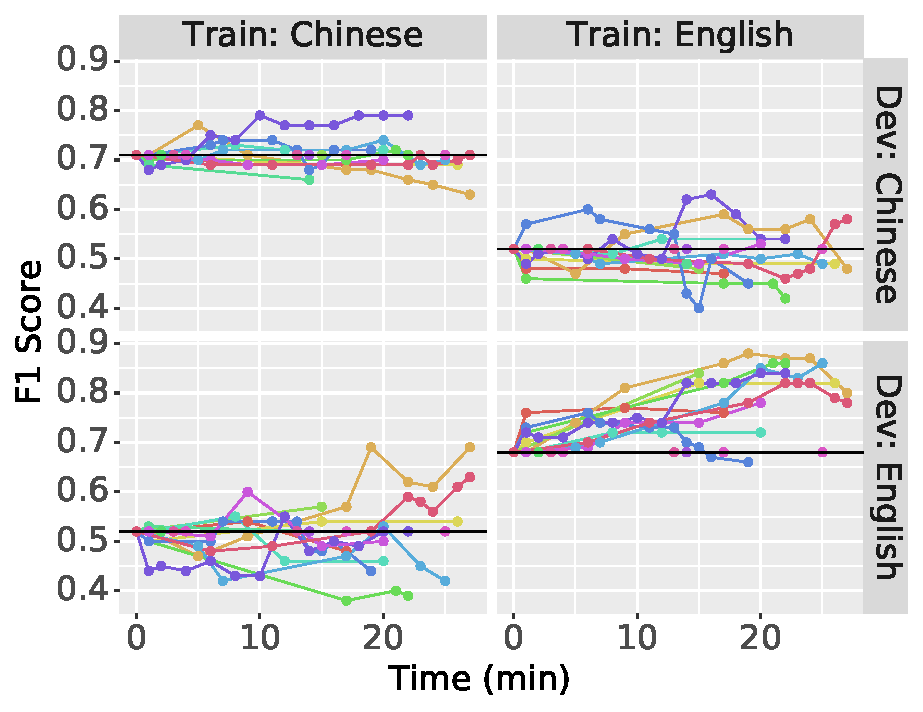
\includegraphics[width=0.47\textwidth]{userdev.pdf}
  }
  \hfill
  \subfloat{
    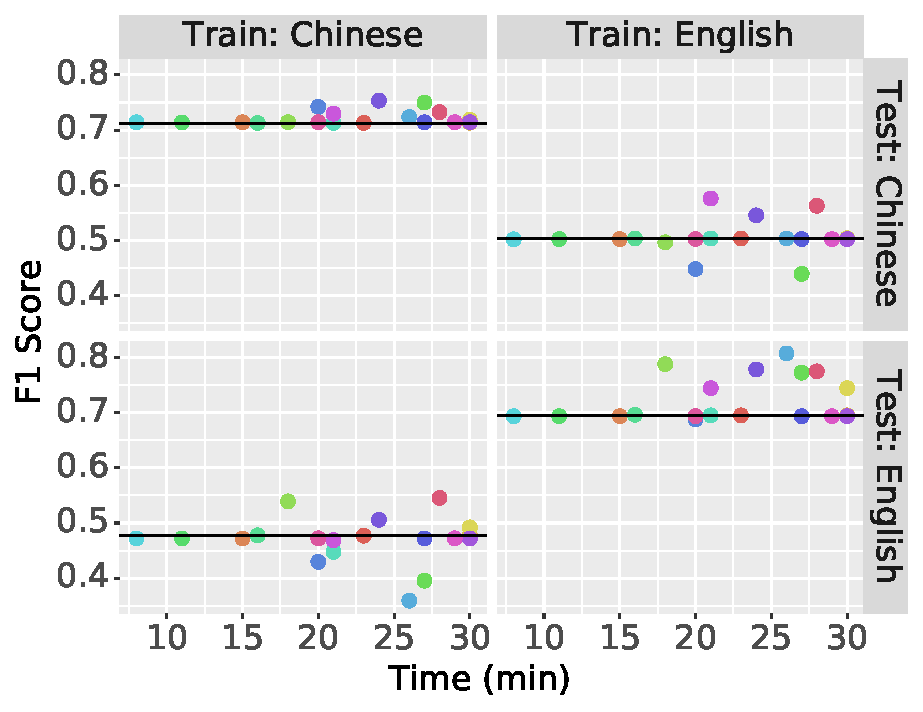
\includegraphics[width=0.47\textwidth]{usertest.pdf}
  }
  \caption{Classification accuracy of each participant in the \mtanchor user study over time.  Each plot indicates the language of topics that the classifier is trained on and the language of topics that the classifier is tested on.  The black horizontal line denotes multilingual anchoring score (no interactive updates).  Each colored line represents a different user interaction and shows the fluctuation in scores on development set (left).  Each colored point represents the final classification score on the test set; the point's x-coordinate indicates total duration of user's session (right).}
  \label{fig:user}
\end{figure}







